%-------------------------------------------------------------------------------
% yum_themes
%-------------------------------------------------------------------------------
%
% \file        yum_themes.tex
% \library     Documents
% \author      Will Godfrey
% \date        2023-05-01
% \update      2023-05-17
% \version     $Revision$
% \license     $XPC_GPL_LICENSE$
%
%     Provides the themes section of the manual.
%
%-------------------------------------------------------------------------------

\section{Themes}
\label{sec:themes}

   \index{Themes}
   \index{themes}
   This section details the new (with \textsl{Yoshimi} V2.3.0) \textbf{Themes}
   feature, that gives access to virtually all colour elements.

\paragraph{Menu / Yoshimi / Settings / Theme}
\label{paragraph:menu_yoshimi_settings_themes}

\begin{figure}[H]
   \centering
   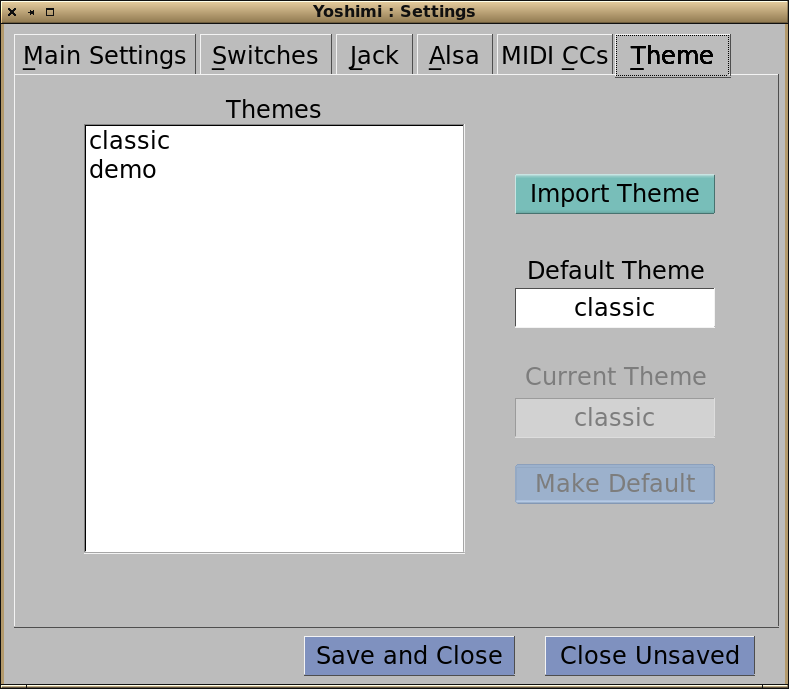
\includegraphics[scale=0.5]{2.3.3/theme.png}
   \caption[Theme Options]{The New Theme Tab}
   \label{fig:yoshimi_settings_themes}
\end{figure}

   The following items are provided by the Theme settings tab:

   \begin{enumber}
      \item \textbf{Installed Themes Menu}
      \item \textbf{Import Theme}
      \item \textbf{Export Theme}
      \item \textbf{Default Theme Display}
      \item \textbf{Current Theme Display}
      \item \textbf{Make Default}
      \item \textbf{Monochrome}
   \end{enumber}

   \setcounter{ItemCounter}{0}      % Reset the ItemCounter for this list.

   \itempar{Installed Themes Menu} {}A click on an entry will immediately switch
   to that theme.

   \itempar{Import Theme} {}Themes can be found via the file manager and
   installed with this button. Any new themes one installs will show in the menu
   next time the window is refreshed.

   \itempar{Export Theme} {}This lets one copy the currently selected theme back
   out for editing in (say) a text editor. This can then be re-imported on top of
   the original, or with a different name to create personalised variations.

   \itempar{Default Theme Display} {}Shows the name of the theme currently set as
   the default one.

    \itempar{Current Theme Display} {}Shows the currently selected theme (which
    may be different to the default).

   \itempar{Make Default} {}Sets the currently displayed theme as the new default
   one.

   \itempar{Monochrome} {}Inverts the current theme to it's grey equivalent. This
   setting is not saved.

\paragraph{Menu / Yoshimi / Themes / Editing}
\label{paragraph:menu_yoshimi_themes_editing}
   Manually editing themes to suit ones own purposes is quite practical, and it
   is for this reason they have been laid out as simple text files.

   Below is part of the 'classic' theme that is provided as a reference file.
   \textsl{Yoshimi} doesn't use this. It is copied out from the internally
   generated values.

   \begin{verbatim}
    Do not edit this. It may be overwritten.
    Instead, copy as template for other named themes.
    Don't add or remove lines between and including dashes.
    This would corrupt the colour map.
    ------------------ data start marker
    0,255, Grey scale min-max (can be reversed) optional + R,G,B, (tint)
    0,255,255, Panels (R,G,B or #rrggbb)
    0,0,0, RESERVED
    186,198,211, Knob shadow (#bac6d3)
    231,235,239, Knob highlight (#e7ebef)
    51,51,51, Knob ring
    0,197,255, Knob ring lit
    61,61,61, Knob pointer default
    225,75,75, Knob pointer changed
    0,0,0, Slider track
    0,170,0, Slider peg default
    ..
    ..
    ..
    255,255,0, Envelope sustain line
    255,255,255, Envelope line
    255,0,0, Envelope line selected
    =================== data end marker
    Add your own notes here:
    Copyright © 2020 A. N. Other
    The default theme
   \end{verbatim}

   As can be seen there is a lot of built-in 'help' text.
   With all colour lines it is important that there are no spaces between the
   number entries themselves, but after the last comma the descriptive text can
   have any characters (or be ommitted).

   The first entry (Grey scale) is placed here as it will significantly affect
   most of the others, so one should decide on this first. Notice it can be
   reversed such that light and dark shades are swapped.

   One can add on three R,G,B values to the greyscale line which will then provide a colour
   tint to elements that have a grey content.

   As an example:

   \begin{verbatim}
    0,255,240,160,80, Grey scale min-max (can be reversed) optional + R,G,B, (tint)
   \end{verbatim}

   This gives a sort of brick-orange tint to everything.

   For all the following entries, and as hinted in the 'Panels', Knob shadow
   and Knob highlight lines, one can use either R, G, B, numbers in the range
   0 to 255, or as hexadacimal entries preceeded with the 'hash' character such
   as '\#090a0b,' which corresponds to '9,10,11,'.

   There is quite extensive error checking, with errors reporting the actual
   line number in the source text. The faulty line and all following ones are
   then ignored.

   In addition to 'classic', there is a 'demo' theme. This uses quite extreme
   settings to give an idea of the range of possibilities. Both of these will be
   kept updated if there are any future additions.

   To allow for updates, a number of 'RESERVED' entries have been included. These
   currently do nothing, but must be kept in place.

\paragraph{Menu / Yoshimi / Themes / Location}
\label{paragraph:menu_yoshimi_themes_location}

   The files are plain text. There is a reference one called 'classic.clr' and a
   rather extreme example called 'demo.clr'.
   'classic' is auto-generated on the first run of the latest yoshimi from github
   or sourceforge. and 'demo' will be transferred from:

   \texttt{/home/user/yoshimi-code/doc/examples/themes}.

   A number of other themes may be added to 'examples' from time to time/

   Their normal location is \texttt{/home/user/.local/share/yoshimi/themes}.

   Since \textsl{Yoshimi} V2.3.3 it has been possible to edit the selected theme
   (with the exception of 'classic') in situ with an external text editor, and for
   as long as the themes window is visible, the changes to the file will be
   immediately activated. Also, the theme list will be immediately updated if one
   adds or removes files from:\\ \texttt{/home/user/.local/share/yoshimi/themes}

%-------------------------------------------------------------------------------
% vim: ts=3 sw=3 et ft=tex
%-------------------------------------------------------------------------------
